\documentclass{article}
\usepackage{ctex}
\usepackage{geometry,ragged2e,setspace,graphicx,verbatim}
\begin{document}
\newgeometry{left=2.5cm,bottom=0cm}
\begin{titlepage}
    \begin{center}
        \setstretch{2}
        
\includegraphics{./50mun.png}\\
        \begin{flushleft}
            \vspace*{3em}
            \normalfont{\zihao{1}\CJKfamily{hei}\bfseries 合肥市五十中第十届模拟联合国大会}\\
            \normalfont{\bfseries \Large\textrm{The 10th Model United Nations of Hefei No. 50 Middle School}}\\
            \vspace*{6em}
            \centering\normalfont{\zihao{0}\CJKfamily{hei}\bfseries 背景文件}
            \\
            \vspace*{3em}
            \centering\normalfont{\Huge\bfseries \textrm{Background Guide}}\\
            \vspace*{5em}
            \centering\normalfont{\zihao{0}\CJKfamily{hei}\bfseries 联合国安全理事会}
            \\
            \vspace*{3em}
            \centering\normalfont{\Huge\bfseries \textrm{United Nations Security Council }}\\
            \vspace*{3em}
            \centering\normalfont{\Huge\bfseries\CJKfamily{hei} 议题:第四次中东战争的调停与善后}\\
            \vspace*{3em}
            \centering\normalfont{\Huge\bfseries\CJKfamily{hei} 作者:模拟联合国社团学术部}
        \end{flushleft}
    \end{center}
\end{titlepage}
\clearpage
\tableofcontents
\clearpage
\part{委员会致辞}
\clearpage
\part{议题介绍}
本次会议的议题是第四次中东战争的调停与善后,包括调停和善后两个方面。历史上1973年10月22日早上,联合国通过了停火决议。本次会议背景设置在停火之前,代表必须先撰写决议草案停战。决议草案的内容包括强制停战撤军、划定联合国管理区域等。该部分预计在第一议程完成。

第二部分是善后,可以包括多方面,如难民、能源问题等。具体可以参考临时议程书。

下面会介绍第四次中东战争的历史与现状。我们将会从第一次世界大战中东格局初步形成,讲到第四次中东战争以色列转败为胜。
\section{历史与现实}
\subsection{第一次世界大战:强弩之末的帝国、现代中东的形成}
\subsubsection{帝国余晖}
一战前的中东版图和现在大不相同,以色列、约旦、叙利亚、沙特阿拉伯等大部分区域处在奥斯曼帝国的统治之下。虽然它们名义上属于奥斯曼帝国统治,但都被英国渗透。如波斯湾沿岸的一些阿拉伯小邦,都任由英国摆布;塞浦路斯和埃及名义上属于奥斯曼帝国,但实际上由英国实际占领和管理。1907年,英国与沙俄签订了《英俄协约》,将阿富汗划进了“势力范围”这让奥斯曼帝国的安全受到威胁,独立地位岌岌可危。

奥斯曼帝国的科技同样和现代世界格格不入。在它的首都,也就是最发达的地区伊斯坦布尔,电灯于1912年才被引进,下水道工程也才刚刚开工。

1908年,青年土耳其党革命开始,试图推翻帝国。在苏丹阿卜杜勒·哈米德二世统治期间,他废除了宪法,解散了议会,试图加强自己的独裁统治。帝国的政治活动被迫转入地下,许多秘密社团应运而生,青年土耳其党就是其中之一。它的初衷是保持帝国领土完整,摧毁独裁专制制度,恢复宪法和议会。虽然苏丹竭力派出警察部队摧毁社团,但也有一些边疆地区无法管控,比如萨洛尼卡,青年土耳其党在这里趁机发展壮大。1908年的一天\footnote{具体日期似乎不可考}青年土耳其党发动了政变,夺取了萨洛尼卡市。1909年他们发动了资产阶级革命,并成功推翻了阿卜杜勒·哈米德二世的独裁专制制度,建立了君主立宪制。

\begin{flushleft}
    \justifying
    \ \ \ \ 但青年土耳其党仍没能拯救奥斯曼帝国,1908年,名义上属于奥斯曼帝国的波黑被奥匈帝国吞并;1911年,意大利夺取了奥斯曼帝国名义上控制的利比亚沿岸地区;1912年,在巴尔干战争中巴尔干同盟击败奥斯曼帝国,夺取了奥斯曼帝国大部分欧洲领土。青年土耳其党明白,自己的大部分地区已被瓜分殆尽,只剩下中东地区。
\end{flushleft}
\centering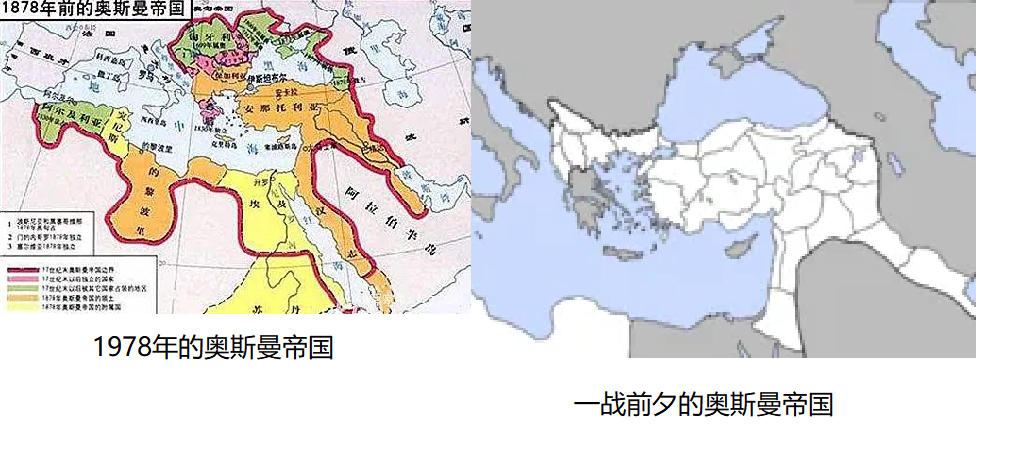
\includegraphics[width=6.4cm]{em.png}\\
\centering \zihao{5} Fig1.1 奥斯曼帝国19世纪末与一战前夕版图对比$^2$\footnotetext[2]{一战前夕意大利与奥斯曼帝国签署了《洛桑条约》,利比亚地区被其实际控制。利比亚也成为意大利在二战中的主要的殖民地}\clearpage
\newgeometry{left=2.5cm,bottom=4cm}
\justifying
\vspace{5pt}
于是,土耳其青年党准备寻找欧洲盟友,哪怕是一个欧洲强国的帮助,都可以让奥斯曼帝国抵御进一步侵略。奥斯曼帝国先找到了英国政府,英国外交部无情拒绝了它的结盟请求。1914年,他们又找到了另外三个欧洲列强:法、德、俄。亲法的奥斯曼海军大臣向法国示好,遭到了拒绝。曾经到过柏林的恩维尔向德国提交的提议又被德国大使拒绝。与俄国的结盟行动最终也遭到了拒绝。奥斯曼帝国遭到了彻底的外交孤立。

此时,英国人还没意识到奥斯曼帝国急切想要一个盟友,英国人还不知道,这直接导致了奥斯曼帝国在第一次世界大战中加入同盟国阵营对英作战。

1914年,欧洲的战争危机愈演愈烈。柏林方面开始重新考虑与奥斯曼帝国的关系。1914年7月24日,德皇威廉二世推翻了德国外交部拒绝与奥斯曼帝国合作的答复,重新考量与奥斯曼结盟的提议。就在前一天晚上,奥匈帝国向塞尔维亚发出了最后通牒,欧洲战争危机即将爆发。1914年8月1日,奥斯曼帝国正式与德国签署同盟协议。协议中包括了奥斯曼帝国最想要的“一旦奥斯曼帝国的领土遭遇威胁,德国有保卫其不受侵犯之义务,必要时应不惜诉诸武力。”,条约还规定了德国向奥斯曼帝国提供军事顾问、物资和财政援助。作为回报,奥斯曼帝国将站在同盟国正式对协约国宣战。

但奥斯曼帝国出于利益,并没有马上对协约国宣战。1914年9月奥斯曼帝国发生了“戈本号”和“布雷斯劳号”事件,让英国开始感到奥斯曼帝国的敌意,但奥斯曼帝国仍没有对英宣战。1914年8月德军发动的坦能堡战役和9月的马祖里湖战役让俄国丢失大量土地,奥斯曼帝国意识到俄国即将输掉战争,如果再不参战,就再也没有机会分到俄国的土地。9月26日,青年土耳其党的军事大臣恩维尔在没有和其他人商量的情况下下令所有船只封锁达达尼尔海峡。这是恩维尔冲动的结果,他将所有筹码都押在了德国上,赌上了帝国的命运。恩维尔下令让“戈本号”和“布雷斯劳号”进入黑海袭击俄国船只。11月3日,英国战舰炮击了达达尼尔海峡要塞,标志着奥斯曼帝国与协约国的战争正式开始。


英国当时的海军大臣,也就是后来二战著名的英国首相丘吉尔从8月份就提出,把奥斯曼帝国当成英国敌人是有好处的。战争发起后,英国终于开始考虑肢解奥斯曼帝国并把领土许配给其他国家。几个世纪以来,欧洲人一直在想肢解奥斯曼帝国后中东的命运将由英国左右,现在英国人终于让历史走上了这一道路。\\
\Large章末问题
\begin{enumerate}
    \small
    \item 末期的奥斯曼帝国和中国哪个朝代很像?为什么?
    \item 为什么奥斯曼帝国末期青年土耳其党掌权仍不能改变奥斯曼帝国的局势?
    \item 奥斯曼帝国应该参加第一次世界大战还是应该中立?为什么?
\end{enumerate}
\subsubsection{协约国介入中东}
\normalsize
\selectfont
英国人在1914年底就开始准备对奥斯曼帝国的瓜分计划。当时的内阁成员斯托尔斯在给盟友法国的信中写到:“英国不会吞并巴勒斯坦地区,但也不会让俄国的势力渗透,或许在巴勒斯坦建立一个犹太国家是最好的方案。犹太人虽然在耶路撒冷占多数,但在整个巴勒斯坦只有1/6的犹太人”但斯托尔斯最终还是认为由埃及吞并巴勒斯坦的方案最好,这也是英国在战时第一次考虑犹太的复国主义。英国于1915年成立了德·本森委员会,这是一个专门制定中东计划的部门。经过讨论,委员会最终决定重新划定中东地区的面貌,中东被分为五个自治省,分别是叙利亚、巴勒斯坦、亚美尼亚、安纳托利亚和贾兹拉—伊拉克。

1915年12月,英国开始筹备入侵中东的计划。但如果英国想调动资源支持中东攻势,必须征得法国的同意。英法两国开始了谈判。法国外交部最希望看到的是由法国直接管理地中海沿岸的黎巴嫩等地区,并通过阿拉伯的傀儡统治者间接控制叙利亚。最终,法国实现了目标,谈判结果规定法国将会统治黎巴嫩地区,并把叙利亚作为法国势力范围---这实际上是为了让法国成为俄国的屏障。但巴勒斯坦的归属仍然不明确,双方都想获得该地区。最终,英国将会获得巴勒斯坦的港口,剩余部分由国际共管。除英法两国控制的地区之外,剩余部分将成立一个阿拉伯国家,尽管这个国家名义上是独立的,但实际上将会在英法两国的势力范围之内。该协议由英国代表M.赛克斯和法国代表G.皮科两名谈判官签订,史称“赛克斯-皮科协定”。
\begin{center}
    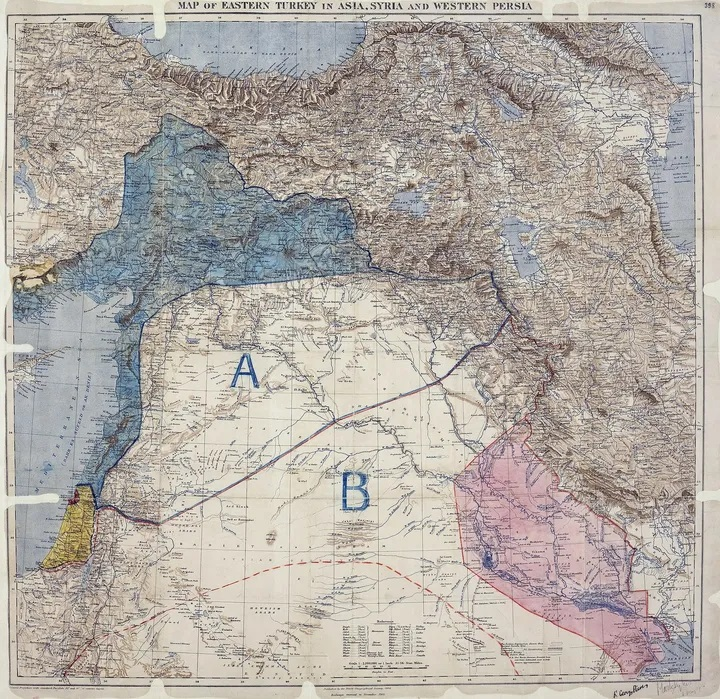
\includegraphics[width=10.4cm]{zd.jpg}\\
    Fig2.1 赛克斯-皮科协定
    \label{fig:Fig2.1}
\end{center}
\clearpage
Fig2.1是赛克斯-皮科协定的示意图。图中叙利亚沿海及黎巴嫩与土耳其的部分地区为“蓝区”,由法国直接占领。伊拉克地区为“红区”,由英国直接占领。巴基斯坦地区为“棕区”,由国际共管。未标注颜色的“A”地区和“B”地区将会成立一个受英法两国控制的阿拉伯国家,国家大小相当于现在的沙特阿拉伯。

1916年2月,两国正式批准该协议。但英法两国一直对协议保密。甚至两年后,外界才知道协约国已对战后中东达成协议。在伦敦,少数几名了解协议的也大多认为该协议对法国让步过多。协议批准过后,英法两国准备将协议给俄国盟友看。在去俄国的路上,赛克斯发现了一个问题。在巴基斯坦的问题上,这份协议考虑到了英法两国的利益,却没有考虑到生活在圣地的犹太人的利益。当时,犹太复国运动已经持续了二三十年,大批犹太人从世界各地回到巴基斯坦定居。如果把巴基斯坦地区交给国际共管,必定会遭到犹太人的反对。

赛克斯很担心,如果他将这个遗漏说给法国人,法国很可能会推翻之前的协议。但其实早在签订协议时,法国人已经注意到这个问题并在3月的法俄秘密会议中与俄国达成一致,将巴基斯坦交给法国人统治。俄国承诺,在之后与英国的谈判中将支持法国提出的巴勒斯坦方案。但英国政府竟一点没有察觉。

俄国人对犹太人没有丝毫同情。赛克斯到俄国后,俄国外交官设法说服赛克斯,让他相信犹太复国主义对协约国是非常危险的。但赛克斯认为,如果协约国想赢得战争,就应该努力安抚犹太复国主义者。不过,犹太复国问题并不是在谈判中的主要问题,谈判主要是为了确定中东的框架。塞尔斯发现俄国的外交官和伦敦的官员看法一样---给法国的实在是太多了。法国大使向俄国大使解释,英国之所以让法国势力范围向东扩展,是为了让法国成为俄国的屏障。这就是英国人的真正想法,英国外交部因为自己想法泄露而后悔莫及,不断向俄国否定。

最终,俄国签署了协定。不过协定实行过程中遭到了很多阻碍,中东划界并没有完全按照协定发展。但《赛克斯-皮科协定》基本奠定了现代中东的雏形。不过,那都是后话了。

\subsubsection{敌后颠覆\ 协约国政府倒台}
一战时中东大小冲突频繁。在波斯,德国人诱使波斯首相签订同盟协议,并取得多个部落的支持。1915年,波斯大部分地区已被这些部落控制。1915年底,俄国军队出兵波斯,并控制了波斯首都,推翻了波斯政府。波斯剩下的清德人员又在其南部建立了一个新政权,并组织军队重新夺回北部。俄国军队在波斯、高加索地区反复和奥斯曼军队拉锯,随意占领波斯领土,一战末期,波斯已不能算一个主权国家。

与此同时,英国也在煽动阿拉伯人起义,因为如果阿拉伯人不起义,《赛克斯-皮科协定》也就无法执行。但阿拉伯对帝国的忠诚超乎英国人的想象,好像帝国就算镇压他们也不会改变自己的忠诚。因此,英国人在阿拉伯地区几乎没有任何进展。英国最后只能寄希望于阿拉伯名族主义分子侯赛因。

1916年6月,侯赛因在汉志发动起义,英国皇家海军迅速在汉志海岸提供海上支持,阻击同盟国军队。侯赛因相信,阿拉伯将会有超过20万人的阿拉伯大起义支持自己,结果并没有发生。奥斯曼帝国军队并没有任何单位倒向侯赛因。几千英国人援助的部队成为侯赛因主力。侯赛因现有的军队根本不是奥斯曼帝国的对手。侯赛因起义发生一年,几乎没有任何进展。《阿拉伯简报》中提出,“侯赛因只是游击队,他们不会进攻土耳其正规军,也顶不住土耳其正规军的进攻”。英国政府给侯赛因支援了4400万美元(现在相当于4亿美元),却没有任何进展。

与此同时,俄国在中东的进展则颇为丰富。1916年,俄国入侵了小亚细亚半岛东部,接着,俄国控制了黑海。德国派往奥斯曼帝国的参谋认为,俄国将会在1917年迫使奥斯曼帝国退出战争。但大量俄国民众在军队服役,导致俄国食品产量低迷;俄国的军火补给线被奥斯曼帝国切断,俄国盟友也没有多少军火能提供给俄国。有人认为,战争实际上已经变成了一场经济和社会层面的生存竞赛。俄国的战时经济拉扯着原有的社会结构,造成俄国社会经济巨大变化。到了1917年,俄国的物价已经上涨了超过10倍。在高加索和德国前线的俄国士兵极度缺乏补给,都饥肠辘辘,在为生存作苦苦挣扎。

最简单的结果方法就是结束战争。1915年,奥斯曼帝国和德国提出,只要俄国退出协约国,它们就准许俄国使用土耳其海峡。在1916年,德国也多次提出和俄国单独议和。但沙皇的帝国野心从未改变。他试图征服奥斯曼帝国,控制土耳其海峡。

弗拉基米尔·伊里奇·乌里扬诺夫,他从1901年开始使用笔名“列宁”,他曾做过律师,后来从事马克思主义事务。1914年,他撰写了《七论战争》,谴责了俄国压迫剥削在波兰、乌克兰的其他名族的行为。他还提出,自己将以俄国战败和解体作为奋斗目标。1916年,彼得格勒饱受食物短缺之苦,在1916-1917年,彼得格勒发动了超过1000次罢工。1917年3月8日,人们为了庆祝妇女节走上街头,发动了一次总人数20万人的罢工。3月15日,俄国沙皇宣布退位,将皇位传给他的弟弟米哈伊尔大公,但他拒绝接受皇位,于是俄国变成了一个由临时政府统治的共和国。1917年秋天,列宁回国并在彼得格勒夺取了政权,建立了苏维埃俄罗斯,他立刻着手让俄国退出战争。1918年3月,俄国接受德国的和平条约,宣布退出战争。俄国退出战争给了协约国沉重一击,同时也是德国和奥斯曼帝国的巨大胜利。
\subsubsection{形势逆转}
到了1916年底,协约国财力已经衰竭,补给品和资金几乎全部依赖美国。1917年,德国的新参谋长保罗·冯·兴登堡和他手下优秀的军事将领对英国发动了无限制潜艇战,即德国潜艇可以不先警告,直接打击英国商船,他认为这样可以快速迫使英国屈服。但这严重损害了美国的利益。


\end{document}